\chapter{The Multiplicative Model}\label{Chapter:MultiplicativeModel}

The Multiplicative Model is one of the infinitely many ways to build stochastic descriptions for SAR data.
Among its advantages we would like to mention that it can be considered an \textit{ab initio} model, and that it leads to expressive and tractable descriptions of the data.

Let us recall that the basic model for multilook intensity data is the $\Gamma(\sigma^2,L)$ law whose density is
\begin{equation}
f_Z(z;L,\sigma^2) = \frac{L^L}{\sigma^{2L}\Gamma(L)} z^{L-1} 
	\exp\big\{ -L z / \sigma^2
	\big\}.
\end{equation}
As previously said, the Gamma distribution is scale-invariant, so we may pose this model as the product between the constant backscatter $X=\sigma^2$ and the multilook speckle $Y\sim\Gamma(1,L)$.

But, are there situations were we cannot assume a constant backscatter?
Yes, there are.

A constant backscatter results from infinitely many elementary backscatterers, i.e.\ from the assumption that $N\to\infty$ in~\eqref{Eq:ComplexBackscatter} (page~\pageref{Eq:ComplexBackscatter}).
Such assumption makes the particular choice of the sensed area irrelevant.
But this may not be the case always.

The advent of higher resolution sensors makes this hypothesis unsuitable in areas where the elementary backscatterers are of the order of the wavelength; cf.\ Table~\ref{Tab:Bands}.
If, for instance, we are dealing with a \SI{1x1}{\meter} resolution image, we may consider $N\to\infty$ if the target is flat and composed of grass;
but if the target is a forest, this assumption may be unrealistic.

\citet{JakemanPusey76} were among the first who tackled this problem.
Assuming that the number of elementary backscatterers $N$ fluctuates according to a Negative Binomial distribution, they obtained a closed-form density which characterizes the $\mathcal K$ distribution:
\begin{equation}
f_Z(z;\alpha,\lambda,L) =
\frac{2\lambda L}{\Gamma(\alpha)\Gamma(L)} (\lambda L z)^{\frac{\alpha+L}{2}-1} K_{\alpha-L}(2\sqrt{\lambda L z}),
\label{Eq:DensKI}
\end{equation}
where $\alpha>0$ measures the roughness, $\lambda>0$ is a scale parameter, and $K_\nu$ is the modified Bessel function of order $\nu$.
This special function is given by $K_\nu (z) = \int_0^\infty e^{-z} \cosh (\nu t) dt$.
See the book by \citet{Gradshteyn80} for other definitions and important properties.
This function is implemented in many numerical platforms as, for instance, in \texttt R.

We denote $Z\sim \mathcal K(\alpha,\lambda,L)$ the situation of $Z$ following the distribution characterized by~\eqref{Eq:DensKI}.
The $k$-order moments of $Z$ are
\begin{equation}
E(Z^k) = (\lambda L)^{-k} \frac{\Gamma(L+k)\Gamma(\alpha+k)}{\Gamma(L)\Gamma(\alpha)}.
\label{Eq:MomentKI}
\end{equation}
Eq.~\eqref{Eq:MomentKI} is useful, among other applications, for finding $\lambda^*=\alpha$, the scale parameter that yields a unitary mean distribution for each $\alpha$ and any $L$.

Fig.~\ref{Fig:KIDistribution} shows the densities in linear and semilogarithmic scales of the Exponential and $\mathcal K$ distributions.
They all have unitary mean, and the latter is shown with different degrees of roughness ($\alpha\in\{1,3,8\}$).
It is noticeable that the larger the value of $\alpha$ is, the closer the $\mathcal K$ and $\text{E}$ densities become.
In fact, \citet{frery96} prove that there is convergence in distribution of the latter to the former.

\begin{figure}[hbt]
\centering
\subfloat[Densities]{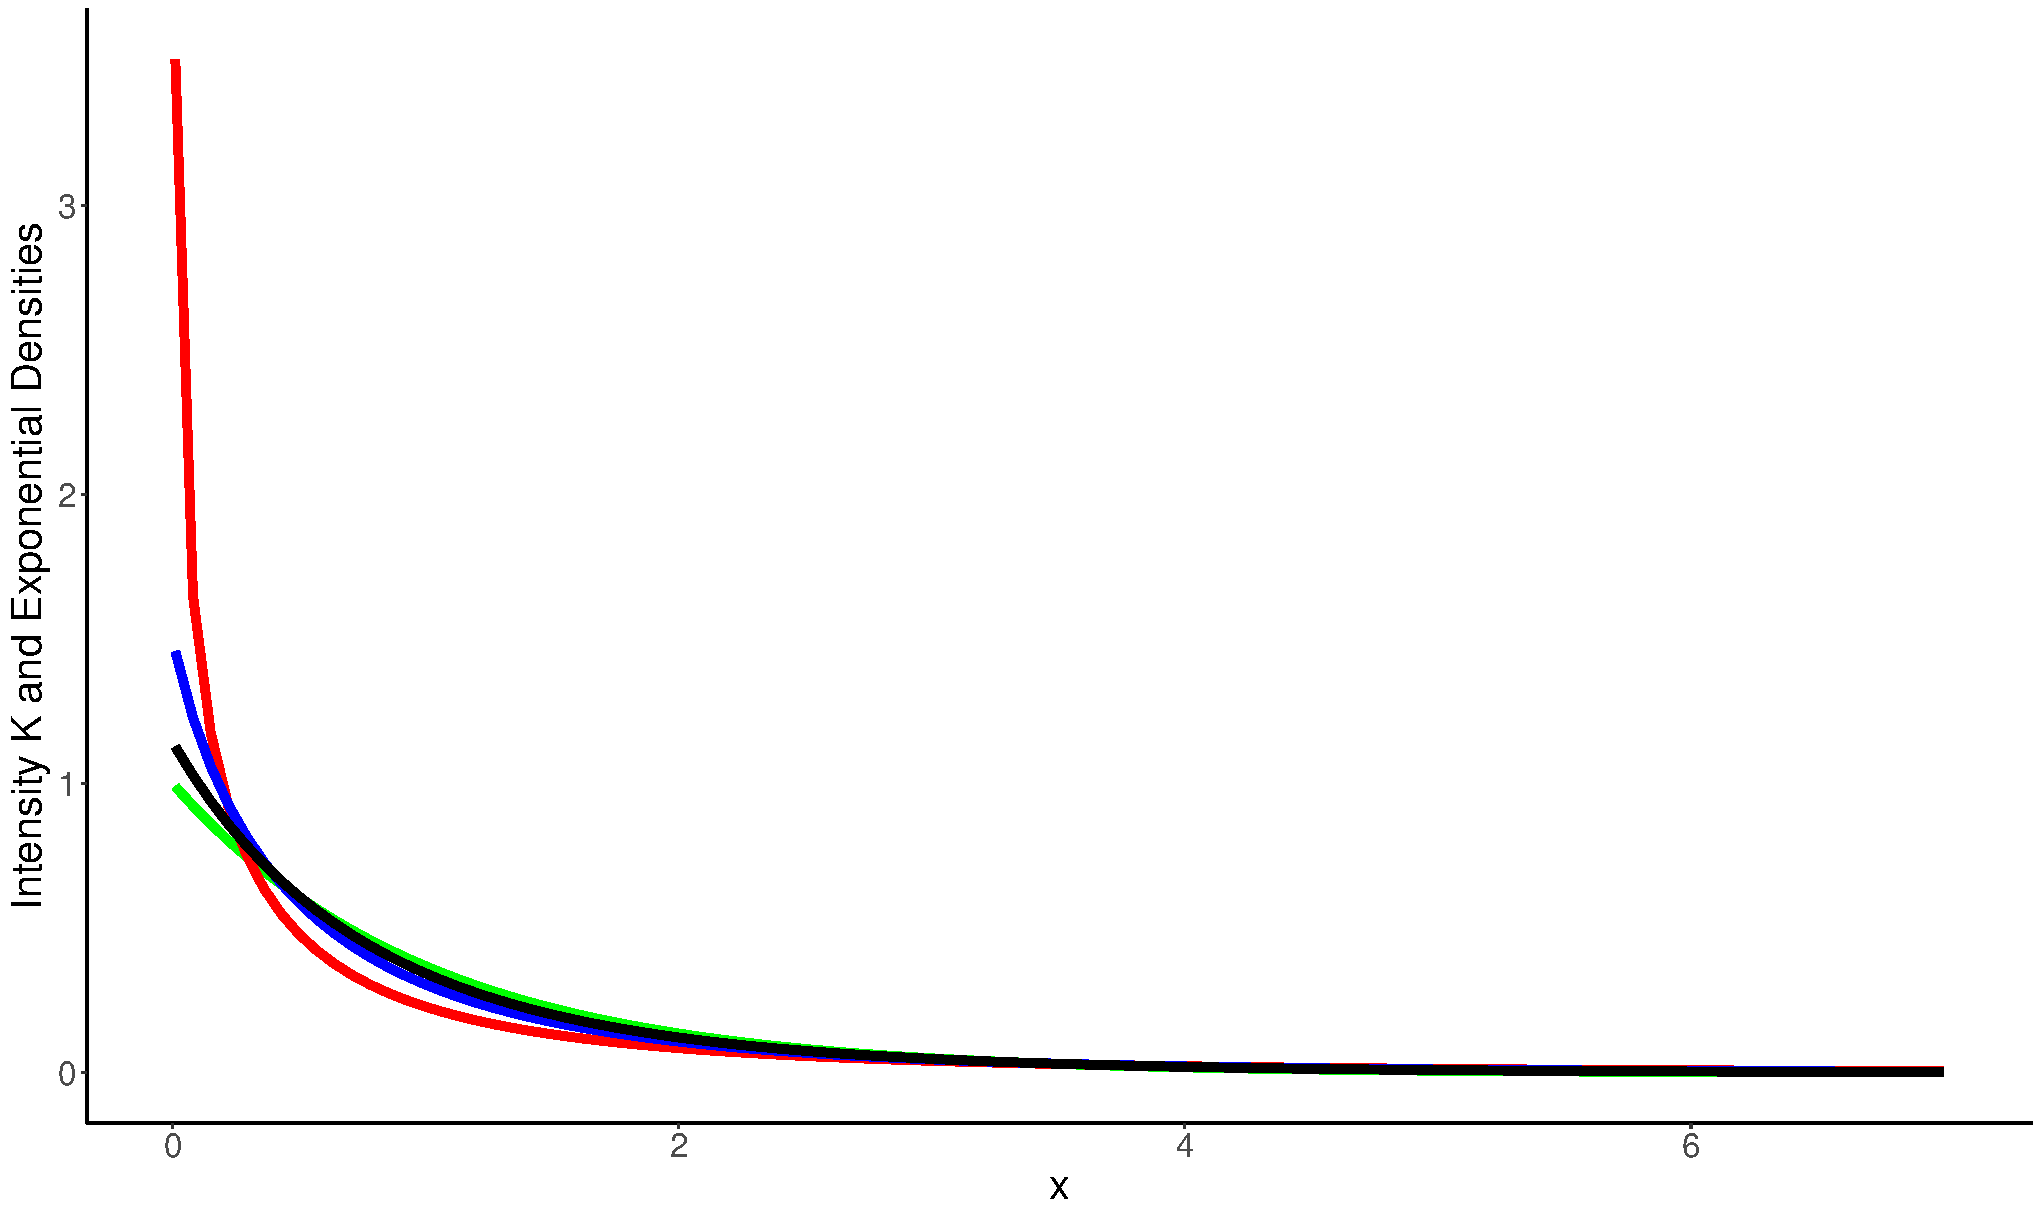
\includegraphics[width=.48\linewidth]{KIDensities}}
\subfloat[Densities in semilog scale\label{Fig:DensKISemilog}]{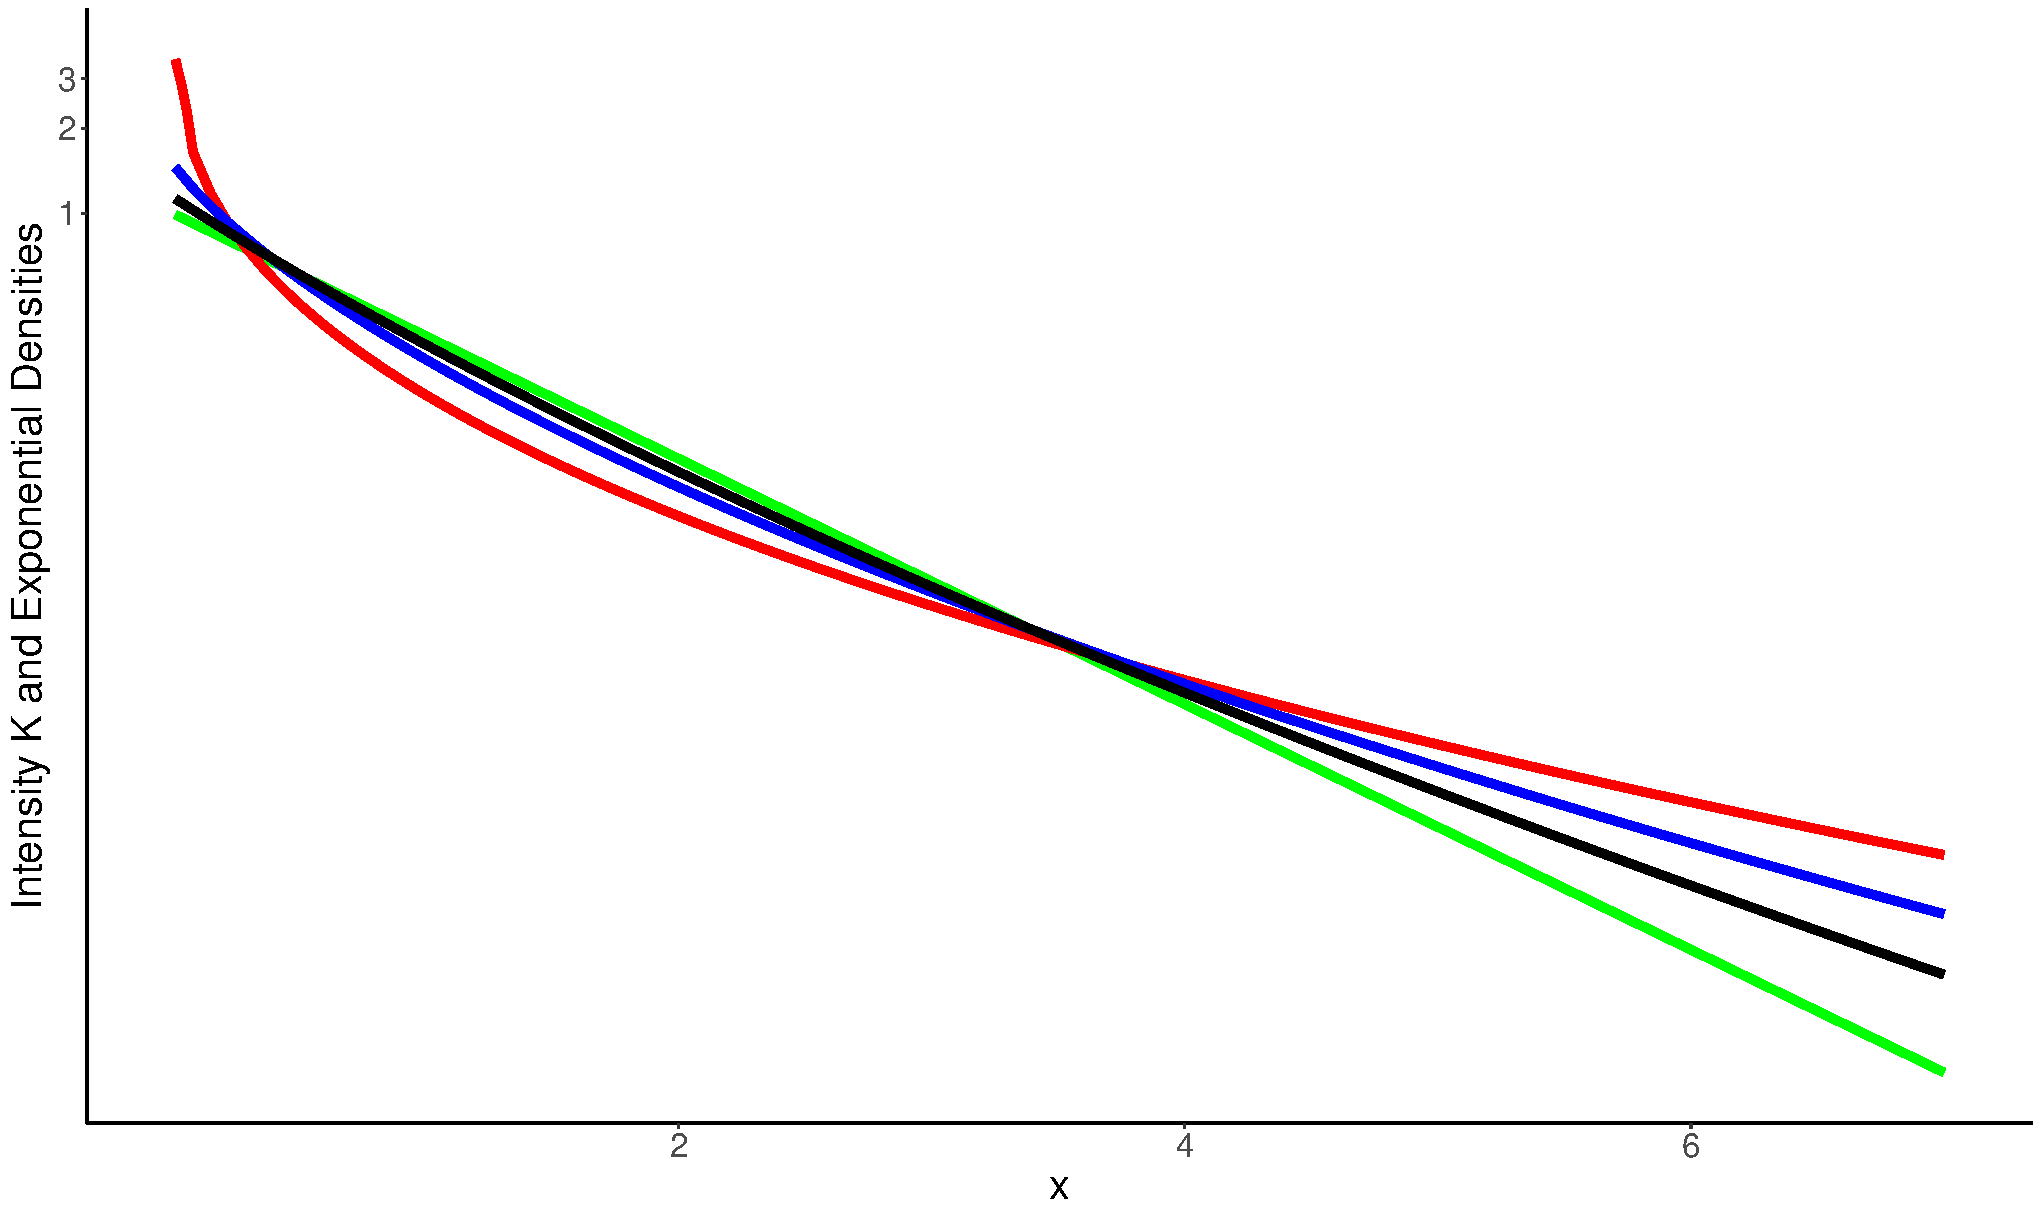
\includegraphics[width=.48\linewidth]{KIDensitiesSemilog}}
\caption{Densities in linear and semilogarithmic scale of the $\text{E}(1)$ (green) and $\mathcal K$ distributions with unitary mean ($\alpha\in\{1,3,8\}$ in red, blue, and black, resp.)}\label{Fig:KIDistribution}
\end{figure}

The difference between these distributions is noteworthy, c.f.\ Fig.~\ref{Fig:KIDistribution}\subref{Fig:DensKISemilog}.
The green straight line is the density of the Exponential distribution, while the red one is that of the $\mathcal K(1,1,1)$ law.
The latter assigns larger probabilities to both small and large values, when compared with the former.
This leads, as will be seen later, to very contrasted data.

Fig.~\ref{Fig:KIDistributionLooks} shows the effect of varying the number of looks, for the same $\alpha=2$ and $\lambda=2$.

\begin{figure}[hbt]
\centering
\subfloat[Densities]{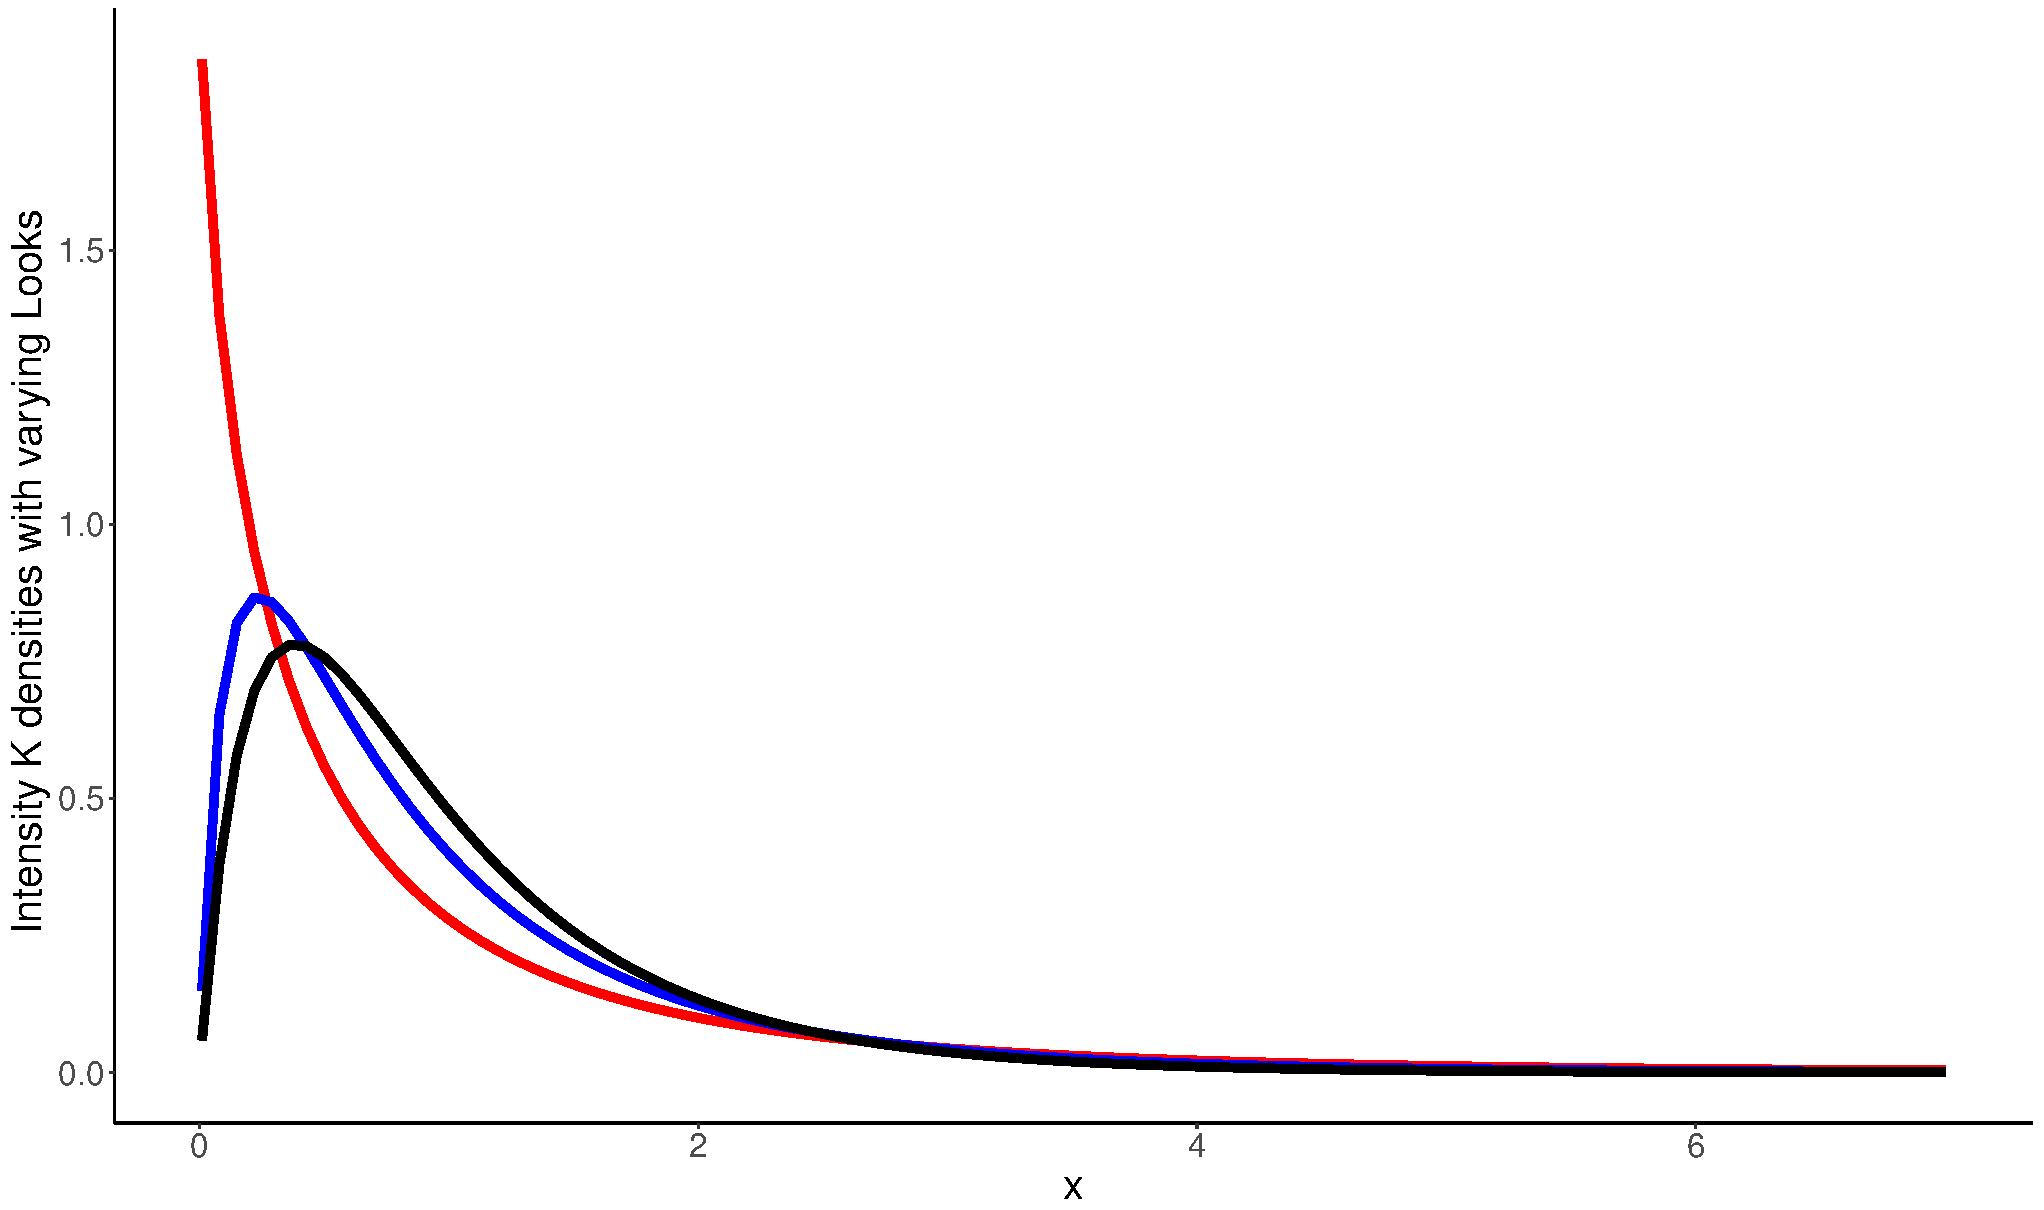
\includegraphics[width=.48\linewidth]{KIDensitiesLooks}}
\subfloat[Densities in semilog scale]{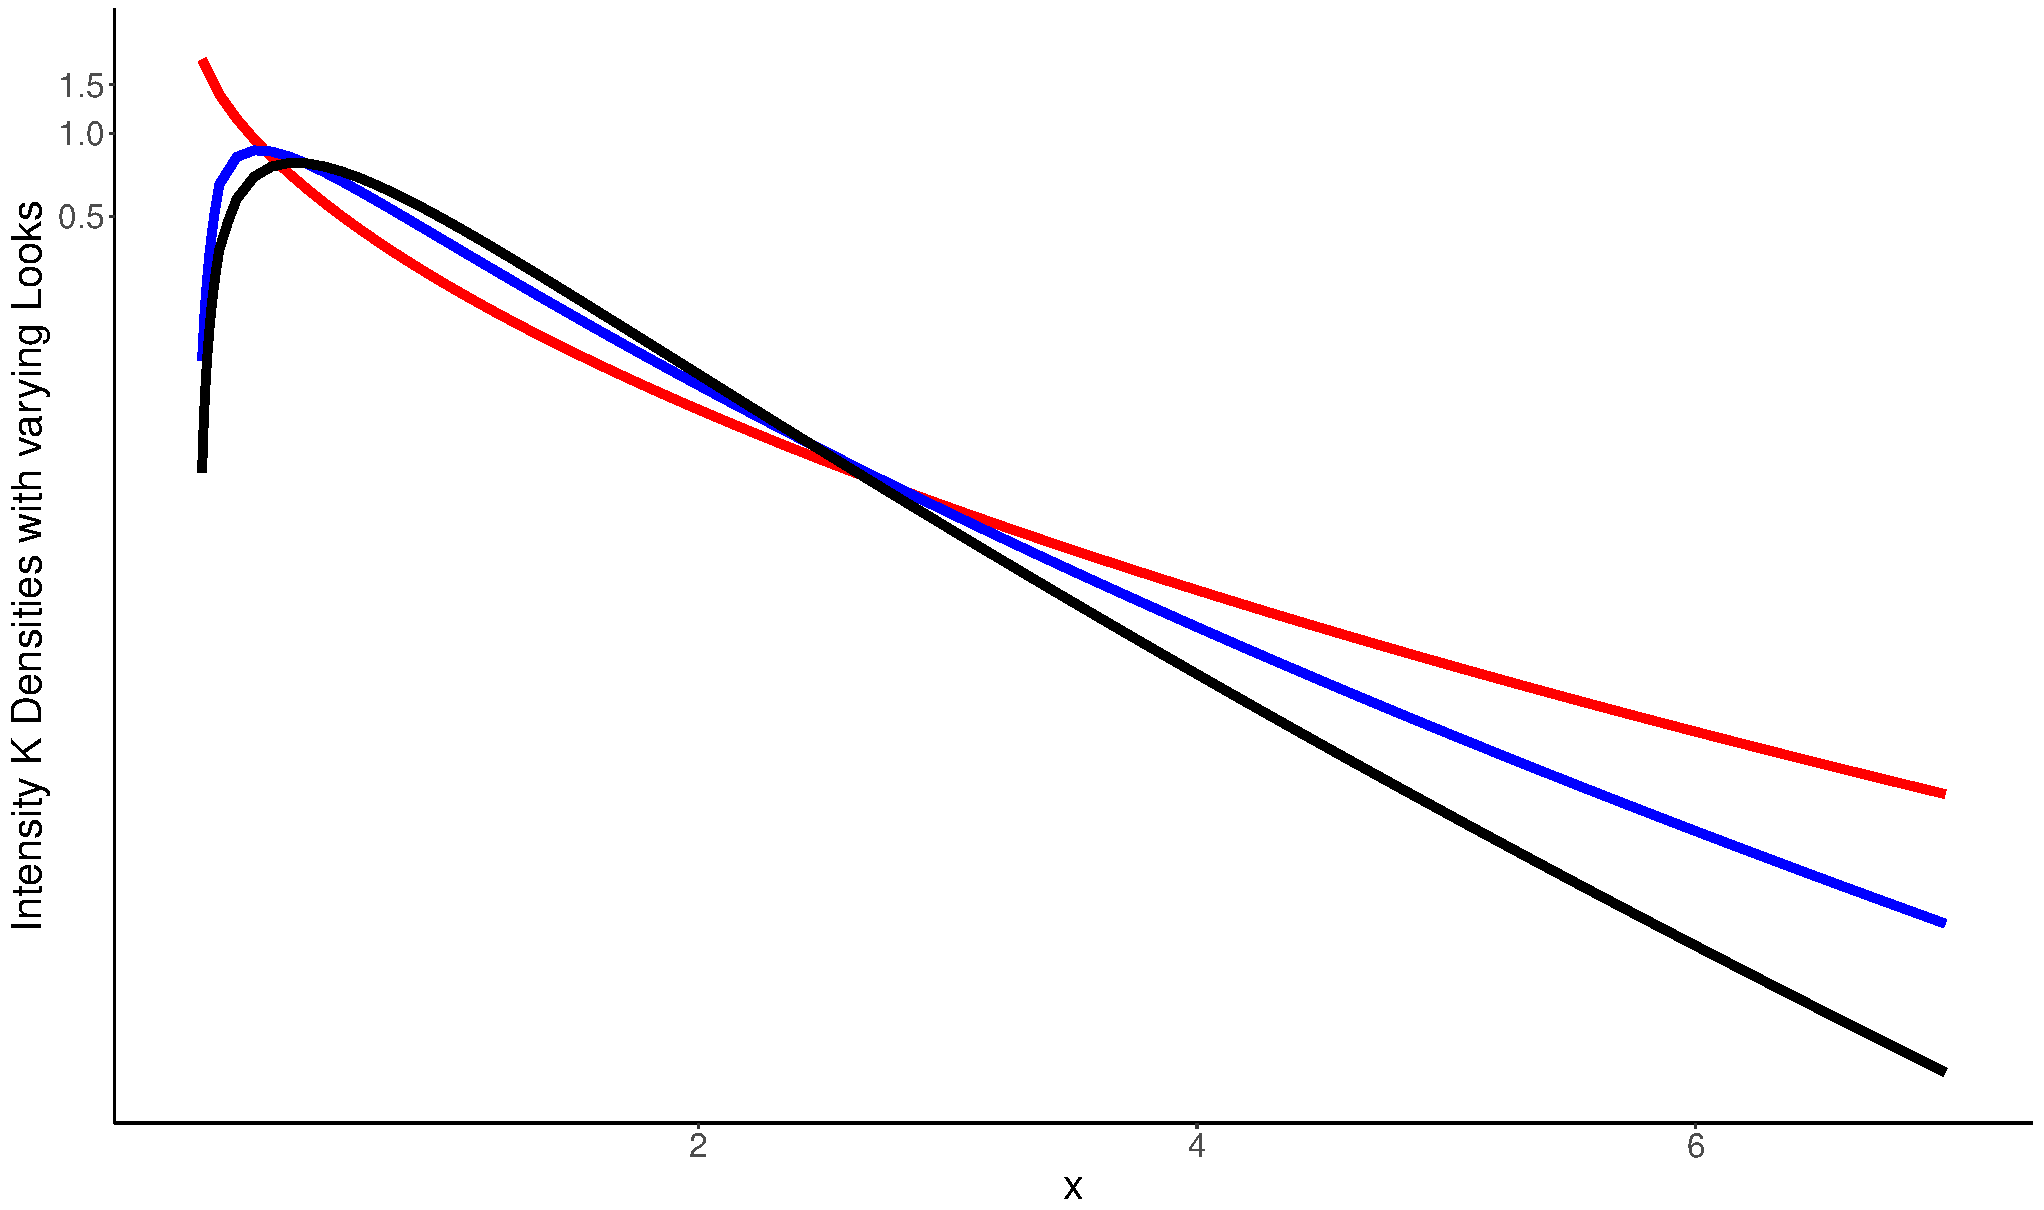
\includegraphics[width=.48\linewidth]{KIDensitiesSemilogLooks}}
\caption{Densities in linear and semilogarithmic scale $\mathcal K)(2,2,L)$ distributions with unitary mean and $L\in\{1,3,8\}$ in red, blue, and black, resp.)}\label{Fig:KIDistributionLooks}
\end{figure}
